
\documentclass[]{beamer}
%%\hypersetup{colorlinks=false}

\usetheme{Singapore}
%%\usetheme{CambridgeUS}

%\usetheme{Hannover}
%% red, blue, brown ou blachandwhite
%%\usecolortheme[named=brown]{structure}
%\usecolortheme{spruce}
%% wolverine ou rose

%\usepackage[french]{babel}
\usepackage[utf8]{inputenc}
\usepackage[T1]{fontenc}

\title{Ce qui nous facilite la vie}
\author{Pierre KURZAWSKI}
\date{3 Novembre 2015}

\begin{document}

\maketitle

\section{Titre de section pour apparaitre dans le plan}
\begin{frame}{Ce qui nous facilite la vie}

  \begin{block}{Plan}
  \begin{itemize}
  \item Organisation
  \item Planning
  \item Choix du design
  \item Présentation du code
  \item Difficultées rencontrées
  \item Conclusion
  \end{itemize}
  \end{block}
\end{frame}

\begin{frame}{Organisation}
  \begin{itemize}
  \item Répartition du travail
  \begin{itemize}
  \item Contenu : à 2
  \item Structure HTML : bibi
  \item CSS : Fricotin
  \end{itemize}
\end{frame}


  \begin{itemize}
  \item Échange du code
  \begin{itemize}
  \item Via GitHub
  \end{itemize}
  \end{itemize}

  \begin{itemize}
  \item Écriture du rapport et du diaporama
  \begin{itemize}
  \item Via Framapad
  \end{itemize}
  \end{itemize}




  \end{itemize}
  \end{block}
\end{frame}

\begin{frame}{Planning}
	\item Semaine 1 & 2 : CHoix de design et récolte des informations
	\item Réalisation de la version 0
	\item Mise en commun et débuggage
	\item Réalisation de la version finale
	\item Finalisation du rapport
	\item Préparation de la soutenance
\end{frame}

\begin{frame}{Présentation du code}
  \begin{center}
    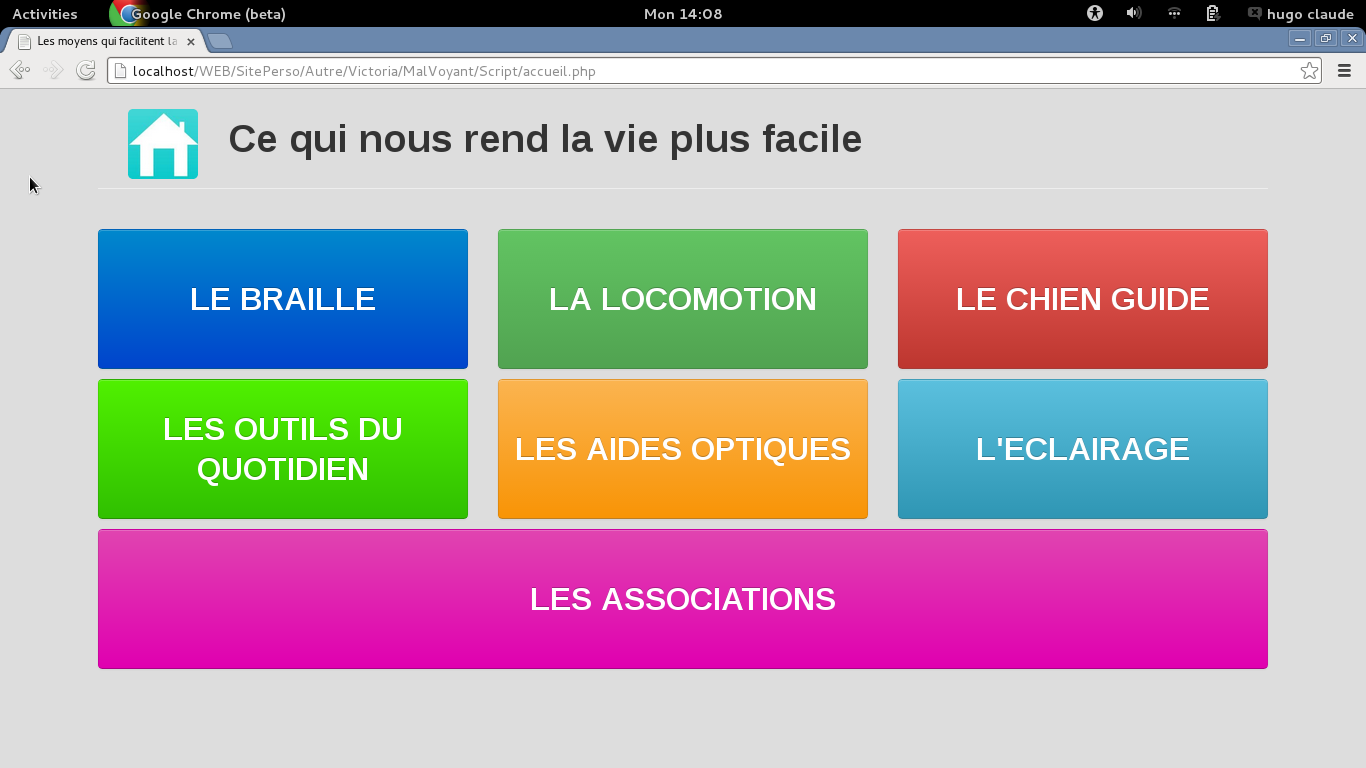
\includegraphics[height=6cm]{site.png}
  \end{center}
\end{frame}

\begin{frame}{Présentation du code}
  \begin{center}
    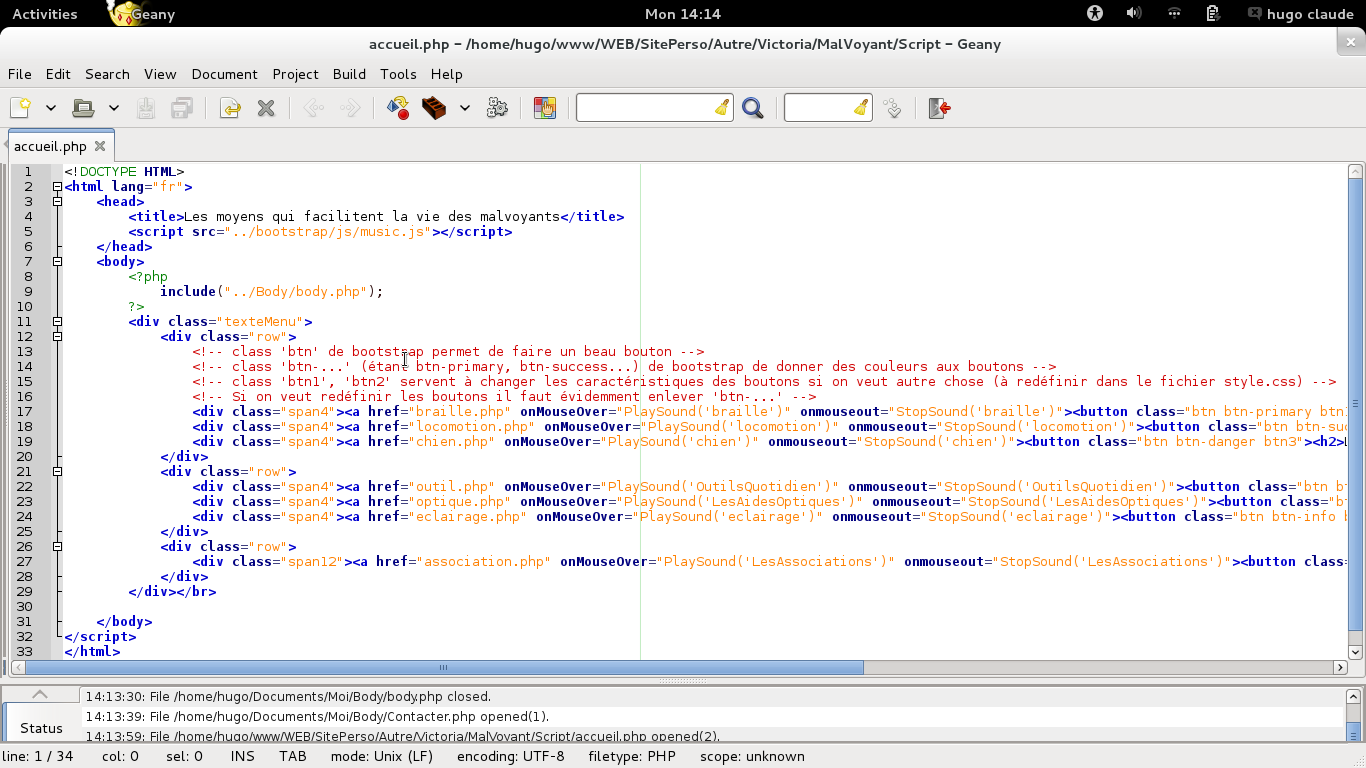
\includegraphics[height=6cm]{code.png}
  \end{center}
\end{frame}

\begin{frame}{Planning}
	\item Compréhension du code
	\item Cohésion de l'ensemble du projet
	\item Compatibilité des navigateurs
	\item Temps insuffisant
\end{frame}

\begin{frame}{Organisation}
  \begin{itemize}
  \item Répartition du travail
  \item Se mettre sur le projet dès le début
  \item Approfondir les notions vues en cours
  \caption{Satisfaction d'avoir réussi un site qui répond au cahier des charges}
\end{itemize}
\end{frame}

\end{document}
